\newpage
\subsection{Integrators}
\label{sec:integrators}
In Mitsuba, the different rendering techniques are collectively referred to as 
\emph{integrators}, since they perform integration over a high-dimensional
space. Each integrator represents a specific approach for solving
the light transport equation---usually favored in certain scenarios, but
at the same time affected by its own set of intrinsic limitations.
Therefore, it is important to carefully select an integrator based on 
user-specified accuracy requirements and properties of the scene to be 
rendered. 

In Mitsuba's XML description language, a single integrator
is usually instantiated by declaring it at the top level within the
scene, e.g.
\begin{xml}
<scene version=$\MtsVer$>
	<!-- Instantiate a unidirectional path tracer,
	     which renders paths up to a depth of 5 -->
	<integrator type="path">
		<integer name="maxDepth" value="5"/>
	</integrator>

	<!-- Some geometry to be rendered -->
	<shape type="sphere">
		<bsdf type="diffuse"/>
	</shape>
</scene>
\end{xml}

This section gives a brief overview of the available choices 
along with their parameters.

\subsubsection*{Path length}
\begin{figure}[htb!]
\centering
\hfill
\smallrendering{Max. length = 1}{pathlength-1}
\smallrendering{Max. length = 2}{pathlength-2}
\smallrendering{Max. length = 3}{pathlength-3}
\smallrendering{Max. length = $\infty$}{pathlength-all}
\caption{
	\label{fig:pathlengths}
	These Cornell box renderings demonstrate the visual 
	effect of a maximum path length. As the paths
	are allowed to grow longer, the color saturation
	increases due to multiple scattering interactions
	with the colored surfaces. At the same time, the
	computation time increases.
}
\end{figure}

Almost all integrators use the concept of \emph{path length}.
Here, a path refers to a chain of scattering events that 
starts at the light source and ends at the eye or camera.
It is often useful to limit the path length (\figref{pathlengths}) 
when rendering scenes for preview purposes, since this reduces the amount 
of computation that is necessary per pixel. Furthermore, such renderings
usually converge faster and therefore need fewer samples per pixel.
When reference-quality is desired, one should always leave the path 
length unlimited.

\begin{figure}[h!]
\centering
\vspace{-5mm}
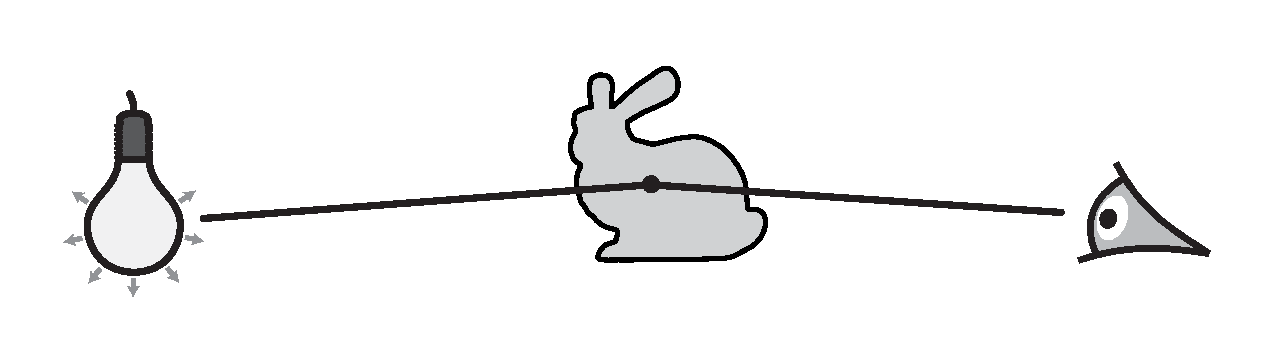
\includegraphics[width=10cm]{images/path_explanation.pdf}
\vspace{-5mm}
\caption{
	\label{fig:path-explanation}
	A ray of emitted light is scattered by an object and subsequently 
	reaches the eye/camera.
	In Mitsuba, this is a \emph{length-2} path, since it has two edges.
}
\end{figure}
Mitsuba counts lengths starting at $1$, which correspond to
visible light sources (i.e. a path that starts at the light 
source and ends at the eye or camera without any scattering 
interaction in between).
A length-$2$ path (also known as ``direct illumination'') includes
a single scattering event (\figref{path-explanation}).

\subsubsection*{Progressive versus non-progressive}
Some of the rendering techniques in Mitsuba are \emph{progressive}.
What this means is that they display a rough preview, which
improves over time. Leaving them running indefinitely will
continually reduce noise (e.g. in Metropolis Light Transport)
or both noise and bias (e.g. in Progressive Photon Mapping).

